\documentclass[english,11pt]{article} 
\usepackage[margin=1in]{geometry}
\usepackage{multicol}
\usepackage{lipsum}
\usepackage{graphicx}
\bibliographystyle{plain}
\usepackage[hidelinks]{hyperref}
\usepackage[utf8]{inputenc}
\usepackage{babel}
\usepackage[T1]{fontenc}
\usepackage{textcomp}
\usepackage{lmodern, newunicodechar}
\usepackage{textgreek}
\usepackage{url}
\usepackage{enumitem}
\usepackage{minted}
\usepackage{amsmath}
\usepackage{mathtools}
\usepackage{mathrsfs}
\usepackage{sistyle}
\usepackage{csvsimple}

\begin{document}

\begin{titlepage}

\begin{center}
        
\includegraphics[scale=0.1]{LOGO-UNIV-FC_COULEUR.png}
        \hspace{1cm}
        
\includegraphics[scale=0.05]{utinam.png}\\
        \vspace{1cm}
\end{center}\\
    \vbox{ }

    \vbox{ }

    \begin{center}
        % Øverste del av siden
                
        \textsc{\Large HPC Project Report - M2 CompuPhys}\\[1cm]

        % \vbox{ }
        % Tittel
        \noindent\makebox[\linewidth]{\rule{.7\paperwidth}{.6pt}}\\[0.7cm]
        { \Huge \bfseries Multi-Threaded N-Body Simulation Using OpenMP and OpenACC}\\[0.25cm]
        \noindent\makebox[\linewidth]{\rule{.7\paperwidth}{.6pt}}\\[0.7cm]
        \LARGE{Léo Bechet}\\[1.2cm]
        
        \vfill
        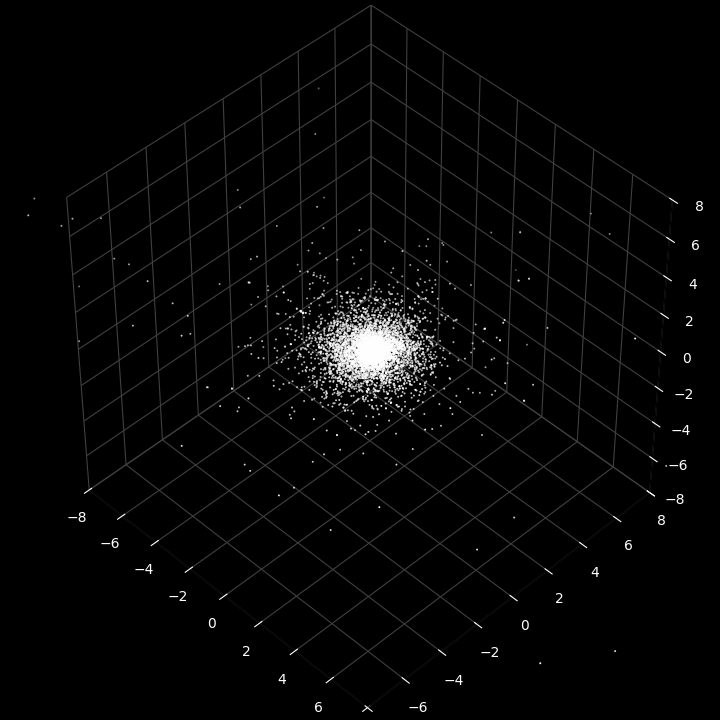
\includegraphics[scale=0.5]{front.png}\\
        \vfill
        % Forfatter
        \large
        % \emph{Skrevet av:}\\[1mm]
        \textsc{\small Many thanks to Matt from the Fortran Community for his help and expertise.}\\[1cm]

        % Nederste del av siden
    \end{center}
\end{titlepage}

\newpage
\tableofcontents
\newpage




%\textbf{Preliminary Note:} A more in-depth writeup is available and has been provided along with the source code.

\section{Sequential Program}

\subsection{Purpose}
Writing a sequential program first serves as a foundational step in the development process of an N-Body simulation. It allows for verification of the initial assumptions, ensuring that the mathematical models and algorithms are implemented correctly. A sequential program simplifies debugging and provides a baseline for performance comparison when parallelizing the code. Additionally, it enables testing of edge cases, validation of results, and optimization of the computational logic without the added complexity of parallel programming. This step ensures a clear understanding of the program's behavior, which is crucial before introducing parallelization and GPU acceleration.

\subsection{Strategy}

The sequential program is structured to follow the dynamics of an N-Body simulation. Initially, the program loads the initial conditions, including the positions and velocities of all bodies. Accelerations are then computed using Newton's law of motion, presented in Equation (\ref{eq:newton}). The simulation progresses using the leapfrog integration method, which ensures stability and accuracy in long-term evolution.

\begin{equation}
    \mathbf{a}_i = G \sum_{j \neq i} \frac{m_j (\mathbf{r}_j - \mathbf{r}_i)}{\|\mathbf{r}_j - \mathbf{r}_i\|^3},
    \label{eq:newton}
\end{equation}

where $\mathbf{a}_i$ is the acceleration of body $i$, $G$ is the gravitational constant, $m_j$ is the mass of body $j$, and $\mathbf{r}_i$ and $\mathbf{r}_j$ are the positions of bodies $i$ and $j$.

The leapfrog integration is performed in two steps. First, the positions are updated using the velocities and half-step accelerations:

\begin{equation}
    \mathbf{r}_i(t + \Delta t) = \mathbf{r}_i(t) + \mathbf{v}_i(t) \Delta t + \frac{1}{2} \mathbf{a}_i(t) \Delta t^2,
    \label{eq:leapfrog1}
\end{equation}

followed by the velocity update using the new accelerations:

\begin{equation}
    \mathbf{v}_i(t + \Delta t) = \mathbf{v}_i(t) + \frac{\mathbf{a}_i(t) + \mathbf{a}_i(t + \Delta t)}{2} \Delta t.
    \label{eq:leapfrog2}
\end{equation}

This method ensures precise tracking of the system's evolution while maintaining numerical stability. 


\subsection{Energy Conservation}
Energy conservation is a crucial indicator of the quality of an integrator, as it reflects the accuracy and stability of the numerical method in long-term simulations. To assess this, we ran the simulation multiple times, each with thousands of steps, and observed that the total energy remained constant throughout, demonstrating excellent energy conservation. However, it is important to note that regardless of the integrator used, the stability of the simulation also heavily depends on the chosen time step (\( \Delta t \)). An inappropriate \(\Delta t\) can lead to instability or loss of accuracy, highlighting the need for careful selection based on the specific system dynamics. Here we use the sequential code from the OpenMP implementation running using 1 thread.

\begin{figure}[h!]
    \centering
    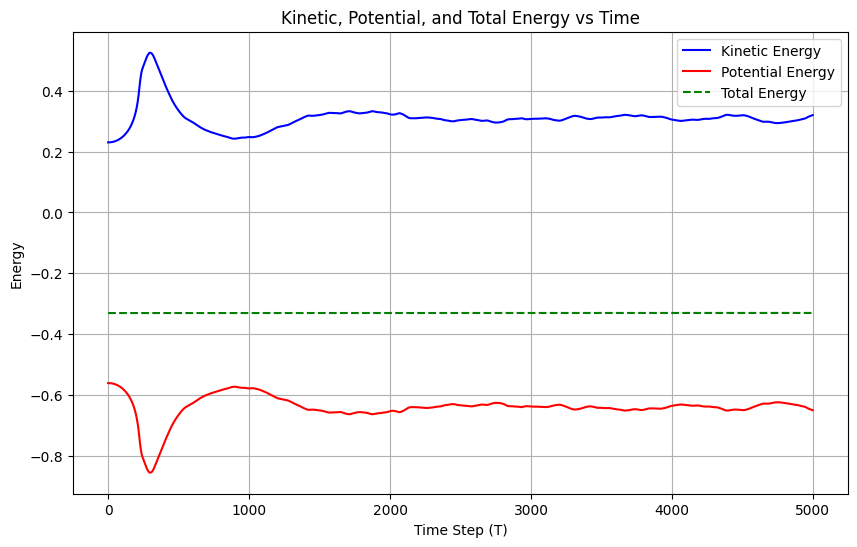
\includegraphics[width=0.6\textwidth]{graph/E_con.png}
    \caption{Energy conservation for a program running on a single thread and parallelism disabled.}
    \label{fig:energy_conservation}
\end{figure}

As shown in Figure \ref{fig:energy_conservation}, the energy remains constant throughout the simulation, confirming that the sequential implementation conserves energy as expected. This validates the correctness of the numerical methods and physical laws used in the program.



\section{OpenMP parallelization}

\subsection{Parallel Zones}

The parallelization strategy began by defining parallel regions for each loop over arrays, focusing on the acceleration computation and the leapfrog updates for positions and velocities. This approach allowed us to test and validate the correctness of each parallelized section independently. Once the prototype was functional, we combined these loops into a single, unified parallel region that also included the time step iteration. 

By merging the loops, the simulation ran within a single, large parallel zone, significantly reducing the overhead associated with the frequent creation and destruction of parallel regions. This optimization is critical for improving performance, as minimizing the parallel zone management overhead allows more computational resources to focus on actual calculations rather than administrative tasks.


\subsection{Private and Shared Variables}
In the parallel implementation, proper management of private and shared variables was essential to ensure correctness and efficiency. During the leapfrog steps, only the loop index needed to be declared as private, as each iteration operated independently on specific elements of the arrays. However, the acceleration computation required several intermediate variables to be private, including those used to calculate distances, force vectors, and potential energy, as these are unique to each thread's computation.

When combining parallel regions into a single large parallel zone, the number of variables involved increased significantly. To manage this complexity, the `default(none)` clause was employed, which required all variables to be explicitly declared as either private or shared. This practice reduced the risk of variables being incorrectly scoped, helping to avoid subtle bugs related to unintended data sharing or overwriting across threads.


\subsection{Qualitative Analysis}
\subsubsection{Energy Conservation}
When comparing the evolution of the energies using either a single thread or multiple threads, the energy remains the same across both implementations. This consistency indicates that the program does not introduce or dissipate energy during the integration process, confirming that the parallelization does not affect the physical accuracy of the simulation. The results are essentially identical, further emphasizing that the parallelized version preserves the integrity of the numerical methods, and the energy conservation principle holds true regardless of the number of threads used.


\subsubsection{Deviation}

The Root Mean Square Deviation (RMSD) and standard deviation (SD) quantify the differences between single-threaded (ST) and multi-threaded (MT) simulations by comparing the distance between the positions of the same particle in both versions. The RMSD, ranging from 0 to 0.005, indicates minimal deviation in particle positions, while the SD between 0 and 0.002 suggests low variation in errors across particles. These results, based on 500 time steps, demonstrate good agreement between ST and MT simulations, with negligible discrepancies. However, longer simulations may show increased divergence due to accumulated numerical errors. These findings are independent of the integrator and time step, as the computations are deterministic.


Figures \ref{fig:rmsd} and \ref{fig:std_dev} show the RMSD and SD, respectively.

\begin{figure}[h!]
    \centering
    \begin{minipage}{0.45\textwidth}
        \centering
        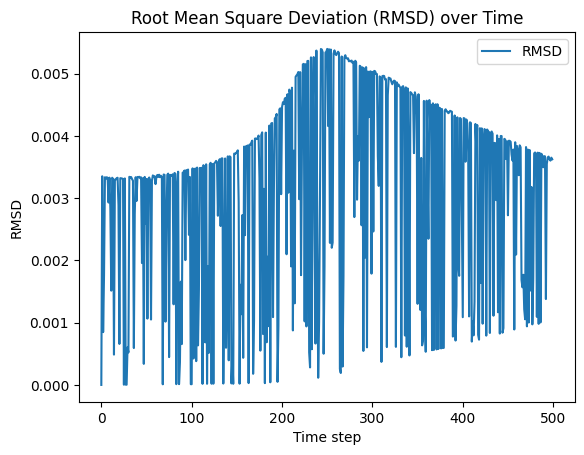
\includegraphics[width=\textwidth]{graph/RMSD.png}
        \caption{RMSD comparison between ST and MT simulations.}
        \label{fig:rmsd}
    \end{minipage}\hfill
    \begin{minipage}{0.45\textwidth}
        \centering
        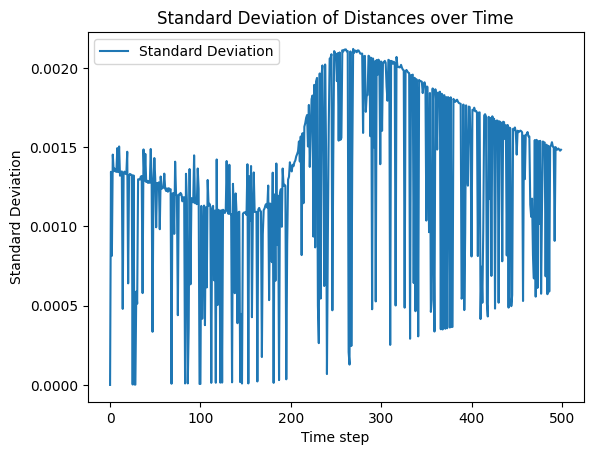
\includegraphics[width=\textwidth]{graph/std_dev.png}
        \caption{SD comparison between ST and MT simulations.}
        \label{fig:std_dev}
    \end{minipage}
\end{figure}





\section{Performance Improvements}
\subsection{Speedup}
The thread-based speed-up plot shown in \ref{fig:speedup} illustrates the program's performance improvement as a function of the number of threads, using the reference execution time determined from the heatmap's optimal settings. As expected, the execution time for a single thread is constant across all scheduling modes. However, the dynamic mode stands out, achieving a significantly higher speed-up compared to other modes.

\begin{figure}[h!]
    \centering
    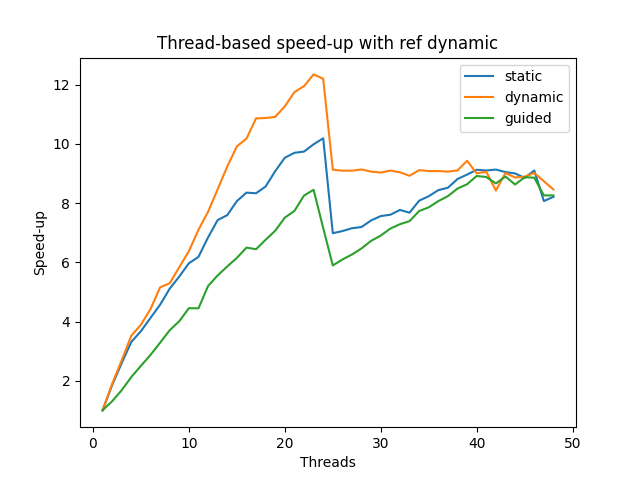
\includegraphics[width=0.6\textwidth]{graph/TB_SU_ref-dynamic.png}
    \caption{Energy conservation for a program running on a single thread and parallelism disabled.}
    \label{fig:speedup}
\end{figure}

We note that past the 23rd thread threshold, performance dips quite dramatically and seems capped. The current understanding blames it on threads competing for shared ressources due to Hyperthreading\footnote{This occurs when multiple threads compete for shared resources, such as the L2 cache, without effective cache sharing mechanisms, leading to reduced performance.}.

\subsection{Efficiency}
Efficiency, defined as the speedup divided by the number of threads, reveals how well parallel computation utilizes available resources. \ref{fig:efficiency} demonstrates a sharp decline in efficiency as the number of threads increases, particularly after the 24th thread, due to resource contention such as L2 cache competition from hyperthreading. Achieving efficiencies above 100\% is rare and requires precise optimization, particularly in data distribution and algorithm tuning. In this case, the efficiency falls short of 100\%, indicating room for further optimization.

\begin{figure}[h!]
    \centering
    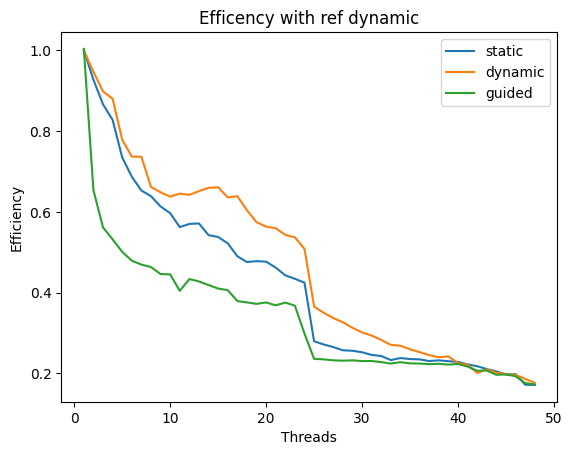
\includegraphics[width=0.4\textwidth]{graph/Efficiency.png}
    \caption{Efficiency comparison as a function of thread count.}
    \label{fig:efficiency}
\end{figure}


\subsection{Thread-Chunk Heatmap}
The Thread-Chunk heatmap visualizes execution times for different scheduling types, highlighting how workload distribution affects parallel performance. When the chunk size is too large, threads become idle, reducing parallelization benefits, as seen in a sharp demarcation line in the heatmaps. This behavior aligns with the throttling observed in the efficiency graph, where performance drops after 24 threads, possibly due to an OS constraint on thread usage. A consistent increase in execution time is also noted for 10 threads, regardless of chunk size.

\begin{figure}[h!]
    \centering
    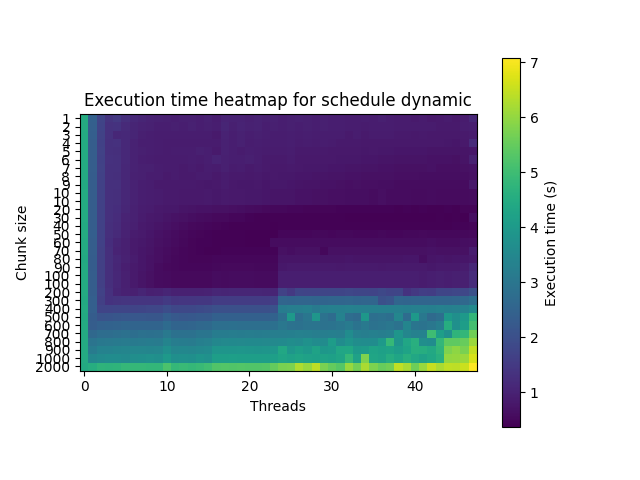
\includegraphics[width=0.5\textwidth]{graph/Heat_dynamic.png}
    \caption{Thread-Chunk Heatmap for the Dynamic shedule.}
    \label{fig:efficiency}
\end{figure}

The optimal configuration, identified by the smallest execution time (0.363417387008667 seconds), is achieved with dynamic scheduling at coordinates (22, 14), corresponding to 23 threads and a chunk size of 50:

\begin{verbatim}
export OMP_SCHEDULE="dynamic,50"
export OMP_NUM_THREADS=23
\end{verbatim}

This configuration optimizes performance by balancing workload distribution. A larger test set of 6000 stars will not be used due to high computation time requirements.


\section{Advanced Optimization}
\subsection{Implemented Techniques}
\subsubsection{Pointers Manipulations}
Instead of swapping data by copying it into another array when advancing to the next step, we use the following subroutine that takes advantage of Fortran's \texttt{move\_alloc()} function to swap pointers efficiently:

\begin{verbatim}
subroutine swap_array(old, new)
    real(kind=8), allocatable, intent(inout) :: old(:,:), new(:,:)
    real(kind=8), allocatable :: temp(:,:)

    call move_alloc(from=old, to=temp)
    call move_alloc(from=new, to=old)
    call move_alloc(from=temp, to=new)
end subroutine swap_array
\end{verbatim}

This method avoids unnecessary data copying by swapping the array pointers, making the operation more efficient.

\subsubsection{Memory management}
To minimize memory usage, we have limited the arrays to four: one for positions, one for velocities, one for current accelerations, and one for the next step accelerations. This approach reduces RAM consumption while efficiently managing the required simulation data. By reusing arrays at different computation stages, we lower the memory footprint and avoid excessive memory usage, which could degrade performance.

\subsubsection{Memory access optimization}
Additionally, the latest version of the code implements position caching for the position of the computed star. This reduces memory access for the position to only the one of the currently compared star.

The same process has been applied to the acceleration computation. We cache the computed force and only add it at the end. This further reduces the number of memory access.



\subsubsection{Asynchronous and Unformatted Saving}
Using unformatted raw data instead of formatted types reduces time consumption by eliminating the overhead of formatting operations. Raw data enables simpler, faster file I/O. 

Asynchronous writing further enhances performance by allowing the program to continue computations while data is written to disk in parallel. Early tests showed a 33\% reduction in execution time with asynchronous writing. However, when the number of threads equals or exceeds the available system threads, diminishing returns occur as asynchronous writing competes with computation threads, negating the performance benefits.




\section{GPU Port}

\subsection{Strategy}

To port the code to the GPU, we eliminated the anti-symmetry in the computations to resolve a race condition that was breaking the code. Atomic operations are necessary to update the acceleration array, and removing the symmetry allowed us to keep the force vector private for each core, updating accelerations individually only once. While we are exploring methods to eliminate the need for atomic operations, no solution has been found yet. Unlike the multi-threaded version, we have not managed to reduce the number of parallel zones, which currently stands at three, leaving room for further optimization to mitigate parallel zone creation overhead, notably by grouping array updates utilizing only the array index for their updates.


\subsection{Qualitative Analysis}

Since we have already demonstrated that the deviation between the MT and ST implementations is negligible, we now compare the MT and GPU implementations. 


\begin{figure}[h!]
    \centering
    \begin{minipage}{0.45\textwidth}
        \centering
        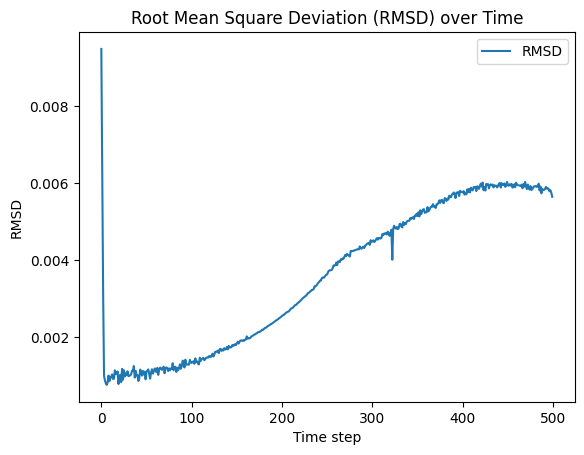
\includegraphics[width=\textwidth]{graph/RMSD_CPU-GPU.png}
        \caption{RMSD comparison between MT and GPU simulations.}
        \label{fig:rmsd_gpu}
    \end{minipage}\hfill
    \begin{minipage}{0.45\textwidth}
        \centering
        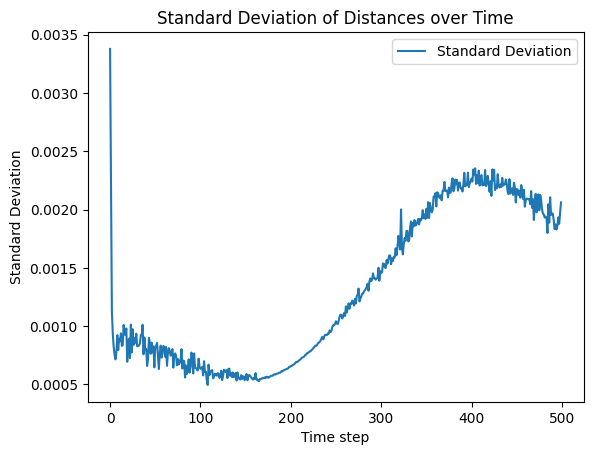
\includegraphics[width=\textwidth]{graph/std-dev_CPU_GPU.png}
        \caption{SD comparison between MT and GPU simulations.}
        \label{fig:std_dev_gpu}
    \end{minipage}
    \begin{minipage}{0.45\textwidth}
        \centering
        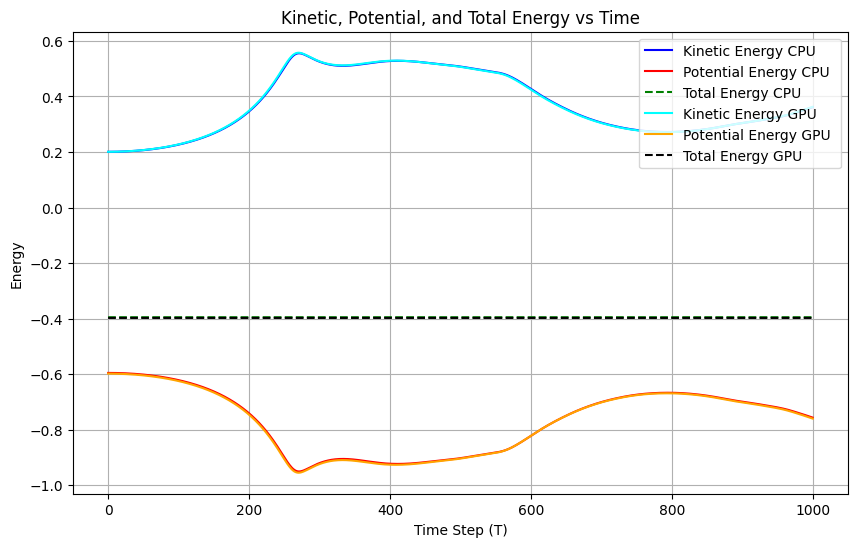
\includegraphics[width=\textwidth]{graph/E_GPUCPU.png}
        \caption{Energy comparison between MT and GPU simulations.}
        \label{fig:E_gpu}
    \end{minipage}
\end{figure}

As shown in \ref{fig:rmsd_gpu} the RMSD between the two remains between 0 and 0.006 over 1000 steps, while the standard deviation in \ref{fig:std_dev_gpu} stays between 0 and 0.0025. These small values indicate minimal discrepancies in particle positions and consistent errors across particles. Furthermore, when superposing the energies from the MT and GPU implementations, they are essentially identical as shown in \ref{fig:E_gpu}. This confirms that the GPU implementation is accurate and produces results consistent with the MT version.


\end{document}






